\chapter{Additional Results}{}
\makeatletter\@mkboth{}{Appendix}\makeatother
\label{appen:additional_results}

This appendix contains the detailed results that are summarised in Chapter~\ref{chap:results}: the full multi-class results of every architecture, the per-facility results of the leave-one-facility-out experiment, the training curves and confusion matrices of the selected models, the augmentation experiment, and the binary results at the chosen thresholds. In every table, the best value in every column is shown in bold.

\section{Experiment 1: Mixed-Facility Baseline}
\label{appen:res_mixed}

\begin{table}[htbp]
\centering
\caption{Clarifier test results of every architecture on the chronological split (Experiment~1). Macro-averaged scores give every class the same weight. The best value in every column is shown in bold.}
\label{tab:res_mixed_clarifier}
\setlength{\tabcolsep}{4pt}
\begin{tabular}{lrrrrr}
\toprule
\textbf{Architecture} & \textbf{Accuracy} & \textbf{Mean AUC} & \textbf{\makecell[r]{Macro\\precision}} & \textbf{\makecell[r]{Macro\\recall}} & \textbf{\makecell[r]{Macro\\F1}} \\
\midrule
ResNet-18 & 0.776 & 0.929 & 0.734 & 0.733 & 0.732 \\
EfficientNet-B0 & 0.780 & 0.927 & 0.679 & 0.715 & 0.691 \\
DenseNet-121 & 0.785 & 0.926 & \textbf{0.798} & \textbf{0.760} & \textbf{0.772} \\
ResNet-50 & 0.761 & 0.922 & 0.715 & 0.699 & 0.702 \\
ConvNeXt-Tiny & \textbf{0.838} & \textbf{0.949} & 0.770 & 0.743 & 0.748 \\
Inception-v3 & 0.773 & 0.926 & 0.692 & 0.724 & 0.706 \\
ResNet-18 (scratch) & 0.713 & 0.904 & 0.650 & 0.704 & 0.667 \\
\bottomrule
\end{tabular}
\end{table}

Table~\ref{tab:res_mixed_clarifier} shows that the macro F1 score of the pretrained clarifier models ranges from 0.691 (EfficientNet-B0) to 0.772 (DenseNet-121). ConvNeXt-Tiny has the highest accuracy (0.838) and mean AUC (0.949). EfficientNet-B0 has the third-highest accuracy but the lowest macro F1 score of the pretrained models, because of its low F1 score for the \textbf{Empty} class (Table~\ref{tab:res_mixed_clarifier_perclass}). ResNet-18 (scratch) has the lowest value in every column except the macro recall.

\begin{table}[htbp]
\centering
\footnotesize
\setlength{\tabcolsep}{3pt}
\caption{Per-class precision (P), recall (R) and F1 score of every clarifier architecture on the chronological split (Experiment~1).}
\label{tab:res_mixed_clarifier_perclass}
\resizebox{\textwidth}{!}{%
\begin{tabular}{l rrr rrr rrr rrr}
\toprule
& \multicolumn{3}{c}{\textbf{Dysfunctional}} & \multicolumn{3}{c}{\textbf{Empty}} & \multicolumn{3}{c}{\textbf{Functional}} & \multicolumn{3}{c}{\textbf{Scum}} \\
\cmidrule(lr){2-4} \cmidrule(lr){5-7} \cmidrule(lr){8-10} \cmidrule(lr){11-13}
\textbf{Architecture} & P & R & F1 & P & R & F1 & P & R & F1 & P & R & F1 \\
\midrule
ResNet-18 & 0.738 & 0.792 & 0.764 & 0.606 & 0.588 & 0.597 & 0.829 & 0.726 & 0.774 & 0.763 & 0.827 & 0.794 \\
EfficientNet-B0 & 0.766 & 0.750 & 0.758 & 0.315 & 0.500 & 0.386 & 0.812 & \textbf{0.863} & 0.837 & 0.823 & 0.746 & 0.782 \\
DenseNet-121 & 0.750 & 0.844 & 0.794 & \textbf{0.846} & \textbf{0.647} & \textbf{0.733} & 0.837 & 0.688 & 0.756 & 0.760 & \textbf{0.859} & 0.806 \\
ResNet-50 & \textbf{0.878} & 0.677 & 0.765 & 0.442 & 0.559 & 0.494 & 0.789 & 0.779 & 0.784 & 0.751 & 0.783 & 0.767 \\
ConvNeXt-Tiny & 0.746 & \textbf{0.885} & \textbf{0.810} & 0.619 & 0.382 & 0.473 & \textbf{0.851} & 0.854 & \textbf{0.852} & \textbf{0.865} & 0.852 & \textbf{0.858} \\
Inception-v3 & 0.757 & 0.844 & 0.798 & 0.415 & 0.500 & 0.453 & 0.809 & 0.763 & 0.785 & 0.788 & 0.788 & 0.788 \\
ResNet-18 (scratch) & 0.775 & 0.823 & 0.798 & 0.352 & 0.559 & 0.432 & 0.687 & 0.829 & 0.751 & 0.786 & 0.607 & 0.685 \\
\bottomrule
\end{tabular}}
\end{table}

Table~\ref{tab:res_mixed_clarifier_perclass} shows that the \textbf{Empty} class has the lowest F1 score of every architecture, from 0.386 to 0.733. The F1 scores of the other three classes range from 0.756 to 0.858 for the pretrained models. The architectures differ most in the \textbf{Empty} precision, which ranges from 0.315 (EfficientNet-B0) to 0.846 (DenseNet-121).

\begin{table}[htbp]
\centering
\caption{Aerobic zone test results of every architecture on the chronological split (Experiment~1).}
\label{tab:res_mixed_aerobic}
\setlength{\tabcolsep}{4pt}
\begin{tabular}{lrrrrr}
\toprule
\textbf{Architecture} & \textbf{Accuracy} & \textbf{Mean AUC} & \textbf{\makecell[r]{Macro\\precision}} & \textbf{\makecell[r]{Macro\\recall}} & \textbf{\makecell[r]{Macro\\F1}} \\
\midrule
ResNet-18 & 0.806 & 0.860 & 0.641 & 0.639 & 0.638 \\
EfficientNet-B0 & \textbf{0.857} & 0.924 & \textbf{0.748} & \textbf{0.733} & \textbf{0.740} \\
DenseNet-121 & 0.813 & 0.898 & 0.663 & 0.664 & 0.662 \\
ResNet-50 & 0.815 & 0.900 & 0.673 & 0.648 & 0.653 \\
ConvNeXt-Tiny & 0.850 & \textbf{0.938} & 0.724 & 0.724 & 0.724 \\
Inception-v3 & 0.820 & 0.903 & 0.696 & 0.683 & 0.687 \\
ResNet-18 (scratch) & 0.781 & 0.893 & 0.625 & 0.624 & 0.624 \\
\bottomrule
\end{tabular}
\end{table}

Table~\ref{tab:res_mixed_aerobic} shows that EfficientNet-B0 and ConvNeXt-Tiny have the highest aerobic zone macro F1 scores (0.740 and 0.724), and the other pretrained models range from 0.638 to 0.687. The accuracy of every architecture is 0.12 to 0.17 higher than its macro F1 score, since the accuracy is dominated by the two large classes and the macro F1 score includes the \textbf{Suboptimal} class. ResNet-18 (scratch) has the lowest accuracy and macro F1 score.

\begin{table}[htbp]
\centering
\small
\setlength{\tabcolsep}{4pt}
\caption{Per-class precision (P), recall (R) and F1 score of every aerobic zone architecture on the chronological split (Experiment~1).}
\label{tab:res_mixed_aerobic_perclass}
\resizebox{\textwidth}{!}{%
\begin{tabular}{l rrr rrr rrr}
\toprule
& \multicolumn{3}{c}{\textbf{Dysfunctional}} & \multicolumn{3}{c}{\textbf{Functional}} & \multicolumn{3}{c}{\textbf{Suboptimal}} \\
\cmidrule(lr){2-4} \cmidrule(lr){5-7} \cmidrule(lr){8-10}
\textbf{Architecture} & P & R & F1 & P & R & F1 & P & R & F1 \\
\midrule
ResNet-18 & 0.817 & 0.932 & 0.871 & 0.911 & 0.818 & 0.862 & 0.196 & 0.167 & 0.180 \\
EfficientNet-B0 & \textbf{0.913} & 0.884 & \textbf{0.898} & 0.875 & \textbf{0.928} & 0.901 & \textbf{0.457} & \textbf{0.389} & \textbf{0.420} \\
DenseNet-121 & 0.854 & \textbf{0.940} & 0.895 & 0.903 & 0.811 & 0.854 & 0.232 & 0.241 & 0.236 \\
ResNet-50 & 0.859 & 0.831 & 0.845 & 0.828 & \textbf{0.928} & 0.875 & 0.333 & 0.185 & 0.238 \\
ConvNeXt-Tiny & 0.877 & 0.916 & 0.896 & \textbf{0.925} & 0.886 & \textbf{0.905} & 0.370 & 0.370 & 0.370 \\
Inception-v3 & 0.809 & 0.900 & 0.852 & 0.915 & 0.852 & 0.882 & 0.364 & 0.296 & 0.327 \\
ResNet-18 (scratch) & 0.852 & 0.811 & 0.831 & 0.849 & 0.875 & 0.862 & 0.172 & 0.185 & 0.179 \\
\bottomrule
\end{tabular}}
\end{table}

Table~\ref{tab:res_mixed_aerobic_perclass} shows that the \textbf{Dysfunctional} and \textbf{Functional} F1 scores range from 0.831 to 0.905, while the \textbf{Suboptimal} F1 score ranges from 0.179 to 0.420. The \textbf{Suboptimal} precision is at most 0.457, so for every architecture fewer than half of the aerobic zones classified as \textbf{Suboptimal} are \textbf{Suboptimal}.

\FloatBarrier

\section{Experiment 2: Leave-One-Facility-Out Evaluation}
\label{appen:res_lofo}

The training curves and confusion matrices are shown for the architecture with the highest mean macro F1 score for each component: ConvNeXt-Tiny for the clarifiers and DenseNet-121 for the aerobic zones.

\begin{table}[htbp]
\centering
\small
\setlength{\tabcolsep}{4pt}
\caption{Clarifier test results of every architecture in the leave-one-facility-out experiment (Experiment~2), given as the mean $\pm$ standard deviation across the five held-out facilities.}
\label{tab:res_lofo_clarifier}
\resizebox{\textwidth}{!}{%
\begin{tabular}{lrrrrr}
\toprule
\textbf{Architecture} & \textbf{Accuracy} & \textbf{Mean AUC} & \textbf{\makecell[r]{Macro\\precision}} & \textbf{\makecell[r]{Macro\\recall}} & \textbf{\makecell[r]{Macro\\F1}} \\
\midrule
ResNet-18 & 0.731 $\pm$ 0.089 & 0.891 $\pm$ 0.033 & 0.770 $\pm$ 0.101 & 0.648 $\pm$ 0.062 & 0.668 $\pm$ 0.068 \\
EfficientNet-B0 & 0.805 $\pm$ 0.093 & 0.931 $\pm$ 0.034 & 0.806 $\pm$ 0.126 & \textbf{0.749} $\pm$ 0.063 & 0.758 $\pm$ 0.098 \\
DenseNet-121 & 0.770 $\pm$ 0.108 & 0.918 $\pm$ 0.025 & 0.767 $\pm$ 0.086 & 0.722 $\pm$ 0.073 & 0.724 $\pm$ 0.086 \\
ResNet-50 & 0.782 $\pm$ 0.115 & 0.911 $\pm$ 0.058 & 0.748 $\pm$ 0.158 & 0.680 $\pm$ 0.149 & 0.681 $\pm$ 0.149 \\
ConvNeXt-Tiny & \textbf{0.838} $\pm$ 0.063 & \textbf{0.953} $\pm$ 0.014 & \textbf{0.861} $\pm$ 0.079 & 0.748 $\pm$ 0.062 & \textbf{0.775} $\pm$ 0.062 \\
Inception-v3 & 0.756 $\pm$ 0.125 & 0.909 $\pm$ 0.046 & 0.799 $\pm$ 0.118 & 0.691 $\pm$ 0.088 & 0.708 $\pm$ 0.109 \\
ResNet-18 (scratch) & 0.735 $\pm$ 0.116 & 0.899 $\pm$ 0.049 & 0.720 $\pm$ 0.109 & 0.666 $\pm$ 0.085 & 0.662 $\pm$ 0.064 \\
\bottomrule
\end{tabular}}
\end{table}

Table~\ref{tab:res_lofo_clarifier} shows that ConvNeXt-Tiny has the highest mean accuracy, mean AUC, macro precision and macro F1 score, and the lowest standard deviation of the accuracy, mean AUC and macro F1 score across facilities. The standard deviation of the macro F1 score ranges from 0.062 (ConvNeXt-Tiny) to 0.149 (ResNet-50). The macro precision is higher than the macro recall for every architecture.

\begin{table}[htbp]
\centering
\small
\setlength{\tabcolsep}{4pt}
\caption{Clarifier test accuracy and mean AUC of every architecture for each held-out facility.}
\label{tab:res_lofo_clarifier_facility}
\resizebox{\textwidth}{!}{%
\begin{tabular}{lrrrrrr}
\toprule
\textbf{Architecture} & \textbf{Atlantis} & \textbf{Cape Flats} & \textbf{Fisantekraal} & \textbf{\makecell[r]{Northern\\Works}} & \textbf{Waterval} & \textbf{Mean} \\
\midrule
\multicolumn{7}{l}{\textit{Accuracy}} \\
ResNet-18 & 0.755 & 0.580 & 0.730 & 0.805 & 0.785 & 0.731 \\
EfficientNet-B0 & \textbf{0.873} & 0.667 & 0.750 & 0.884 & 0.849 & 0.805 \\
DenseNet-121 & 0.800 & 0.599 & 0.738 & 0.854 & 0.859 & 0.770 \\
ResNet-50 & 0.809 & 0.589 & 0.778 & 0.869 & 0.866 & 0.782 \\
ConvNeXt-Tiny & 0.827 & \textbf{0.755} & \textbf{0.806} & \textbf{0.906} & \textbf{0.894} & \textbf{0.838} \\
Inception-v3 & 0.800 & 0.536 & 0.786 & 0.812 & 0.845 & 0.756 \\
ResNet-18 (scratch) & 0.800 & 0.537 & 0.726 & 0.825 & 0.785 & 0.735 \\
\midrule
\multicolumn{7}{l}{\textit{Mean AUC}} \\
ResNet-18 & 0.935 & 0.852 & 0.910 & 0.873 & 0.884 & 0.891 \\
EfficientNet-B0 & 0.965 & 0.882 & 0.915 & \textbf{0.958} & 0.937 & 0.931 \\
DenseNet-121 & 0.941 & 0.876 & 0.926 & 0.926 & 0.920 & 0.918 \\
ResNet-50 & 0.960 & 0.815 & 0.911 & 0.916 & 0.952 & 0.911 \\
ConvNeXt-Tiny & \textbf{0.966} & \textbf{0.938} & \textbf{0.940} & 0.953 & \textbf{0.967} & \textbf{0.953} \\
Inception-v3 & 0.954 & 0.837 & 0.930 & 0.893 & 0.933 & 0.909 \\
ResNet-18 (scratch) & 0.927 & 0.814 & 0.908 & 0.912 & 0.935 & 0.899 \\
\bottomrule
\end{tabular}}
\end{table}

Table~\ref{tab:res_lofo_clarifier_facility} shows that Cape Flats has the lowest accuracy and the lowest mean AUC of every architecture. The accuracy at Cape Flats ranges from 0.536 to 0.755, against 0.726 to 0.906 at the other facilities. ConvNeXt-Tiny has the highest accuracy at four of the five facilities.

\begin{table}[htbp]
\centering
\footnotesize
\setlength{\tabcolsep}{3pt}
\caption{Per-class precision (P), recall (R) and F1 score of every clarifier architecture in Experiment~2, averaged over the held-out facilities at which the class occurs.}
\label{tab:res_lofo_clarifier_perclass}
\resizebox{\textwidth}{!}{%
\begin{tabular}{l rrr rrr rrr rrr}
\toprule
& \multicolumn{3}{c}{\textbf{Dysfunctional}} & \multicolumn{3}{c}{\textbf{Empty}} & \multicolumn{3}{c}{\textbf{Functional}} & \multicolumn{3}{c}{\textbf{Scum}} \\
\cmidrule(lr){2-4} \cmidrule(lr){5-7} \cmidrule(lr){8-10} \cmidrule(lr){11-13}
\textbf{Architecture} & P & R & F1 & P & R & F1 & P & R & F1 & P & R & F1 \\
\midrule
ResNet-18 & 0.743 & 0.623 & 0.675 & 0.821 & 0.461 & 0.553 & 0.722 & 0.695 & 0.667 & 0.785 & 0.756 & 0.745 \\
EfficientNet-B0 & 0.772 & 0.661 & 0.710 & 0.729 & \textbf{0.662} & \textbf{0.649} & \textbf{0.820} & 0.818 & 0.806 & 0.848 & 0.802 & 0.809 \\
DenseNet-121 & 0.786 & 0.728 & 0.754 & 0.634 & 0.560 & 0.565 & 0.780 & 0.777 & 0.749 & 0.823 & 0.763 & 0.773 \\
ResNet-50 & \textbf{0.896} & 0.716 & 0.761 & 0.472 & 0.340 & 0.350 & 0.795 & 0.790 & 0.768 & 0.813 & 0.804 & 0.790 \\
ConvNeXt-Tiny & 0.871 & 0.710 & \textbf{0.776} & \textbf{0.868} & 0.505 & 0.598 & 0.819 & \textbf{0.879} & \textbf{0.836} & \textbf{0.872} & \textbf{0.833} & \textbf{0.843} \\
Inception-v3 & 0.791 & 0.721 & 0.749 & 0.843 & 0.482 & 0.584 & 0.738 & 0.717 & 0.684 & 0.799 & 0.789 & 0.775 \\
ResNet-18 (scratch) & 0.703 & \textbf{0.772} & 0.729 & 0.615 & 0.361 & 0.423 & 0.726 & 0.751 & 0.709 & 0.787 & 0.717 & 0.735 \\
\bottomrule
\end{tabular}}
\end{table}

Table~\ref{tab:res_lofo_clarifier_perclass} shows that the \textbf{Empty} class has the lowest recall for six of the seven architectures, from 0.340 to 0.560. For EfficientNet-B0 it is 0.662, against a \textbf{Dysfunctional} recall of 0.661. The \textbf{Empty} precision is higher than the \textbf{Empty} recall for every architecture, so the main error is that \textbf{Empty} clarifiers are missed, not that other clarifiers are classified as \textbf{Empty}.

\begin{figure}[htbp]
    \centering
    \begin{subfigure}{0.49\textwidth}
        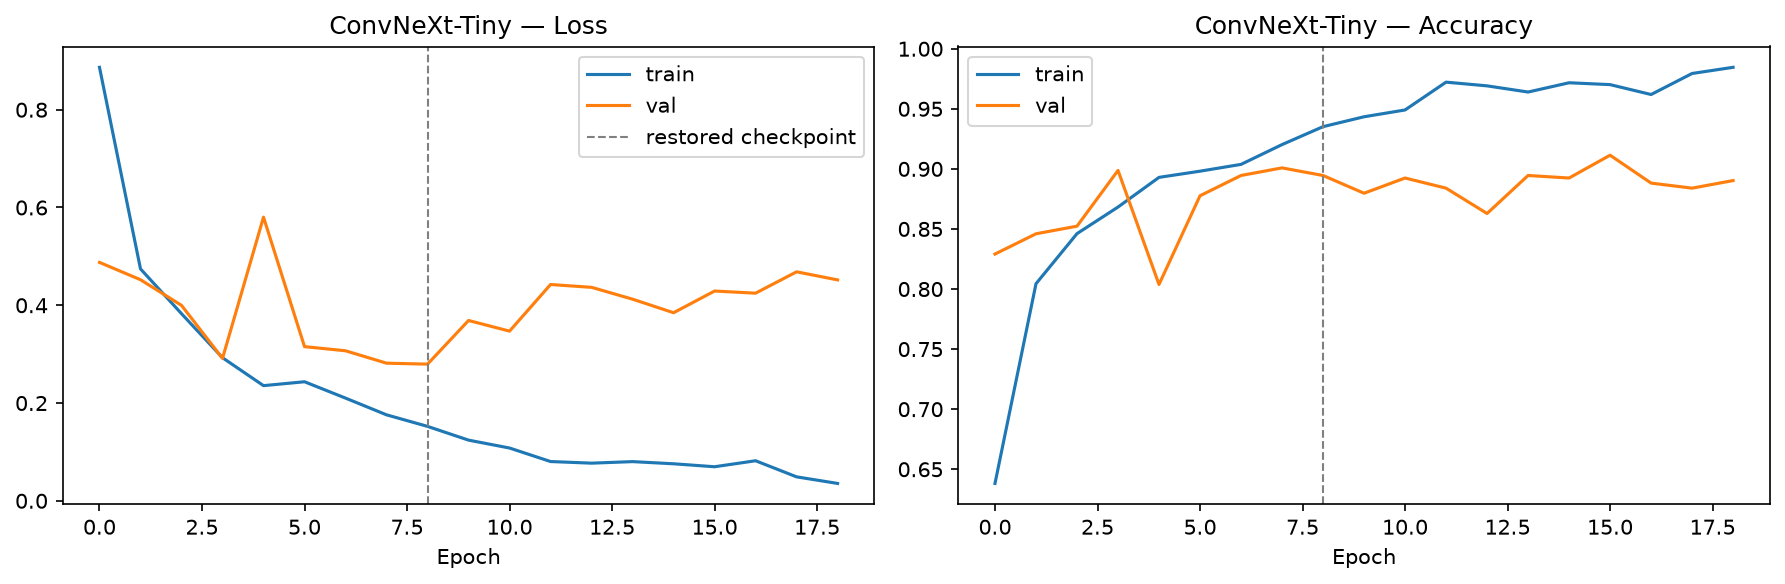
\includegraphics[width=\textwidth]{figures/results/clarifier_convnext_tiny_Atlantis_training_curves.png}
        \caption{Atlantis held out}
    \end{subfigure}
    \hfill
    \begin{subfigure}{0.49\textwidth}
        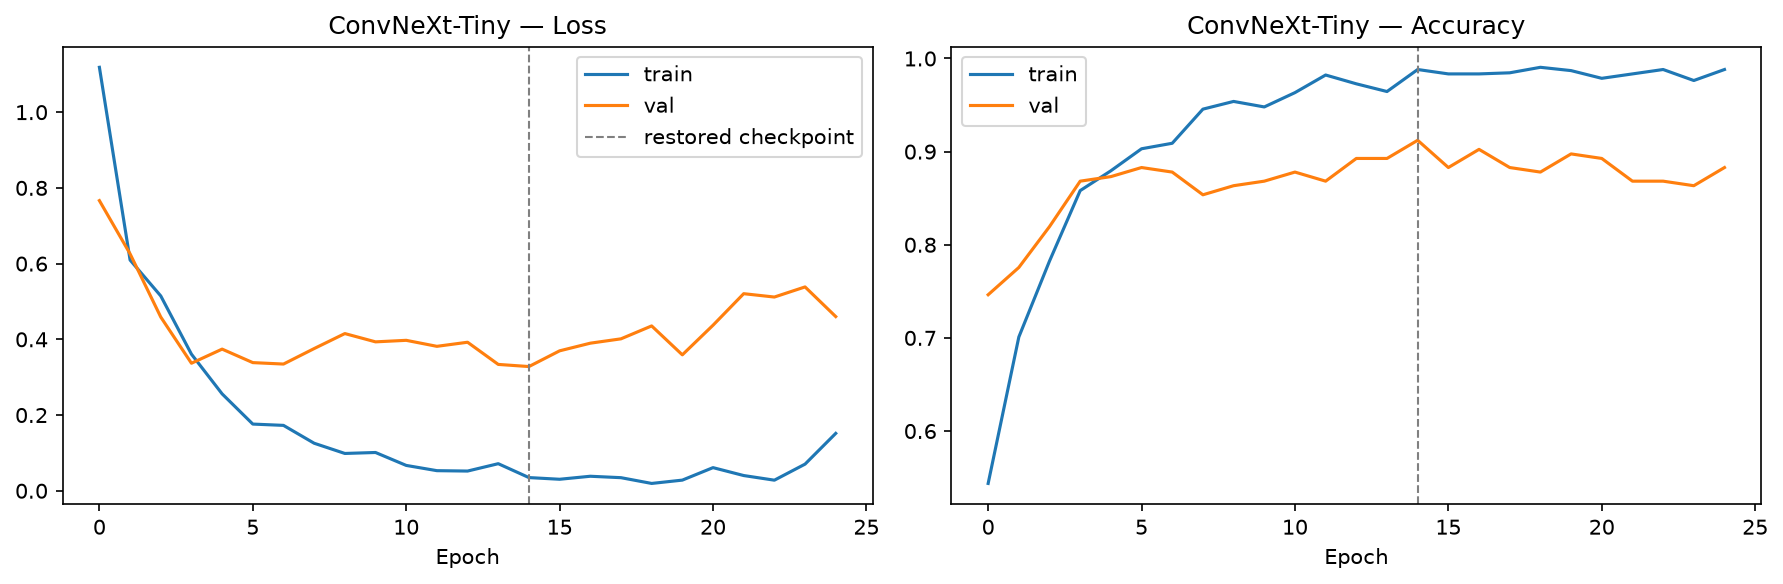
\includegraphics[width=\textwidth]{figures/results/clarifier_convnext_tiny_CapeFlats_training_curves.png}
        \caption{Cape Flats held out}
    \end{subfigure}
    \begin{subfigure}{0.49\textwidth}
        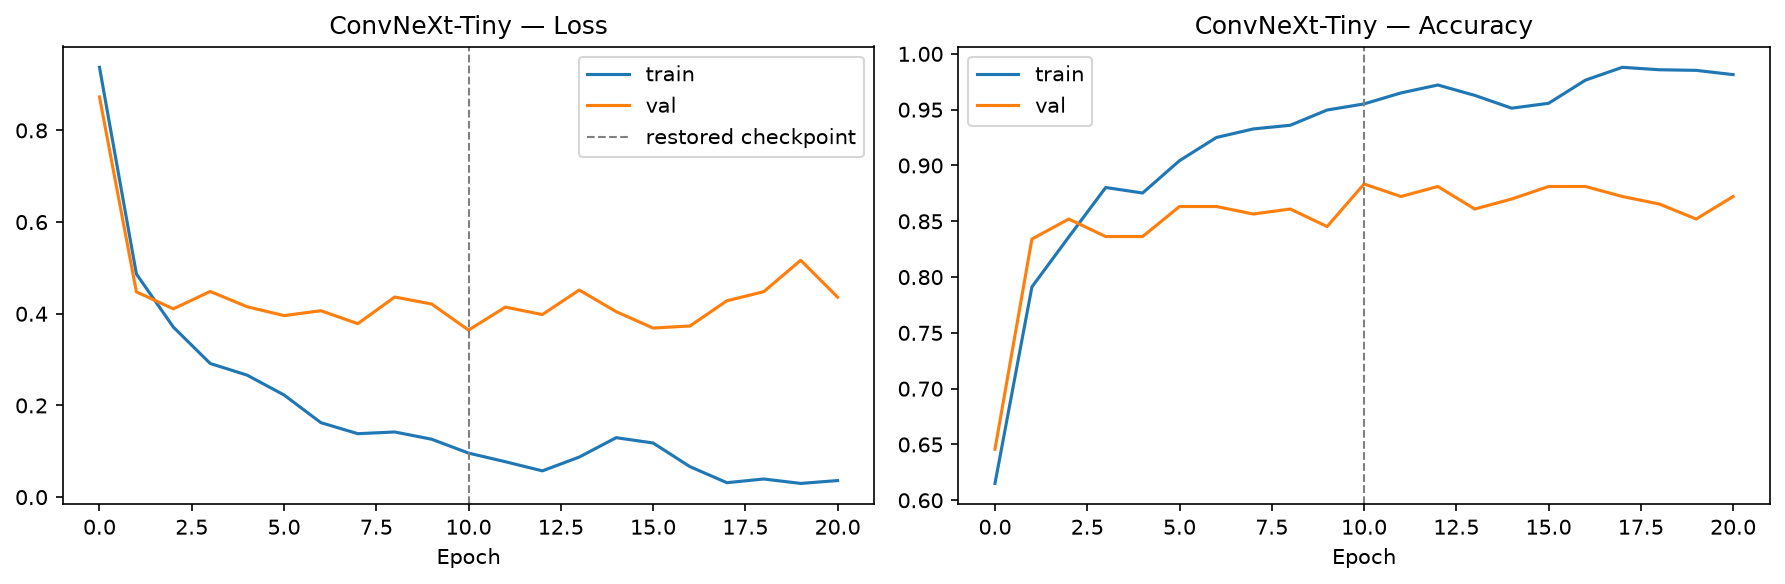
\includegraphics[width=\textwidth]{figures/results/clarifier_convnext_tiny_Fisantekraal_training_curves.png}
        \caption{Fisantekraal held out}
    \end{subfigure}
    \hfill
    \begin{subfigure}{0.49\textwidth}
        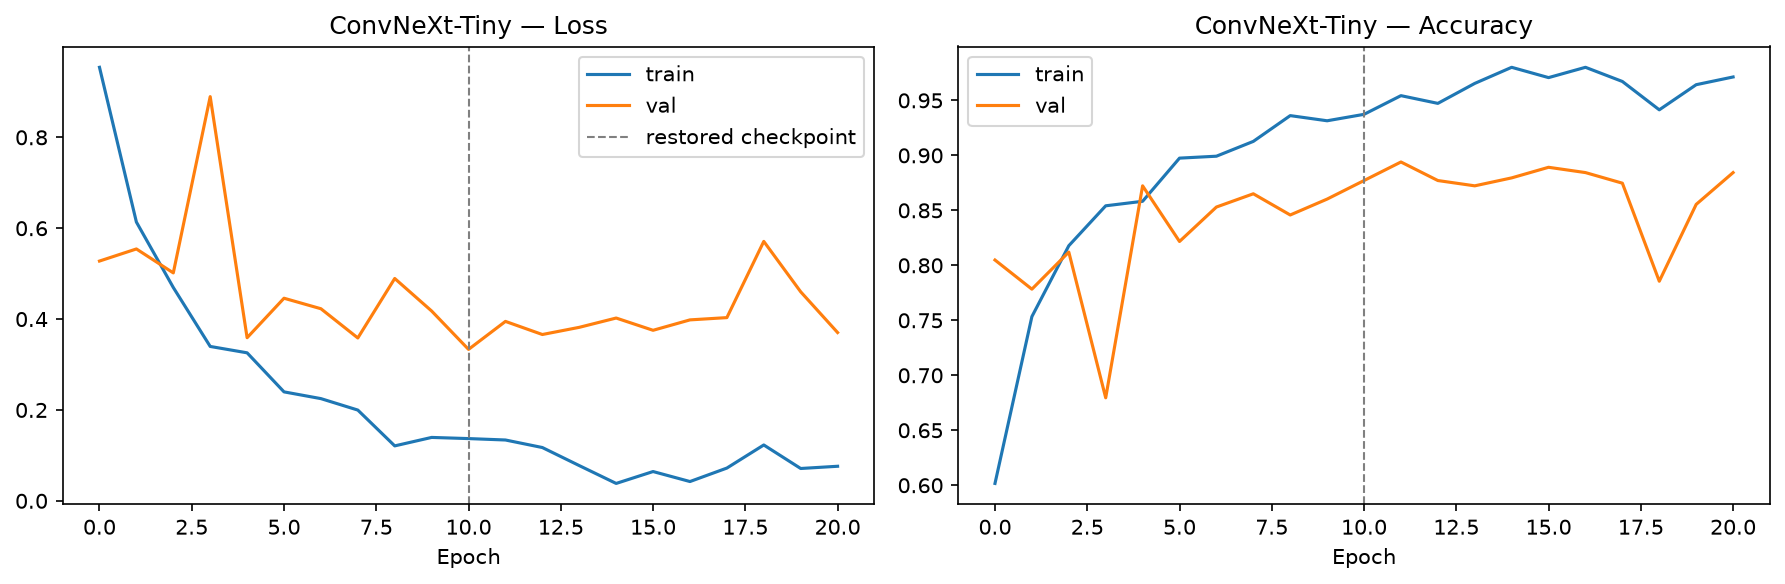
\includegraphics[width=\textwidth]{figures/results/clarifier_convnext_tiny_NoordelikeWerke_training_curves.png}
        \caption{Northern Works held out}
    \end{subfigure}
    \begin{subfigure}{0.49\textwidth}
        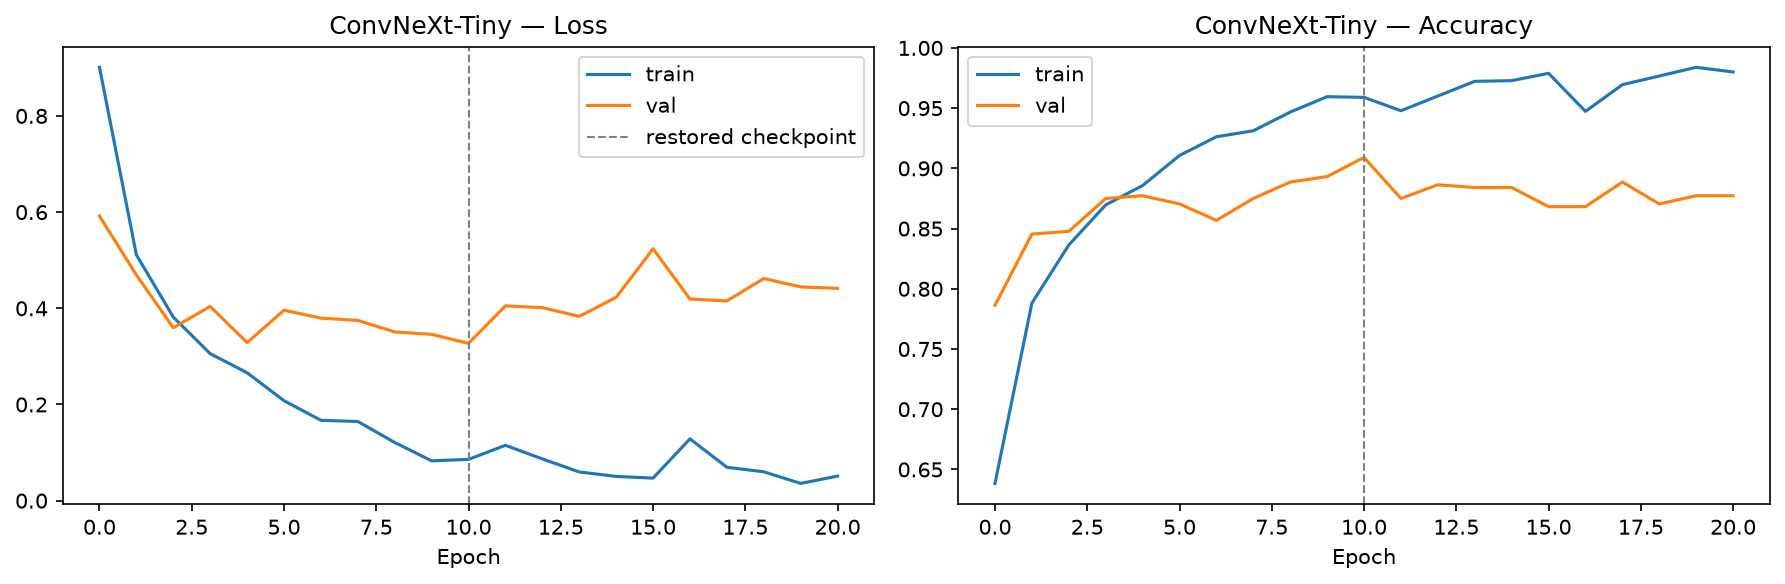
\includegraphics[width=\textwidth]{figures/results/clarifier_convnext_tiny_Waterval_training_curves.png}
        \caption{Waterval held out}
    \end{subfigure}
    \caption{Training and development loss and accuracy of the ConvNeXt-Tiny clarifier model for every leave-one-facility-out fold. The dashed line marks the epoch of the restored checkpoint.}
    \label{fig:res_lofo_clarifier_curves}
\end{figure}

Figure~\ref{fig:res_lofo_clarifier_curves} shows that the development loss of every fold stops decreasing after 9 to 15 epochs, and training stops 10 epochs later, well before the limit of 100 epochs. After the restored checkpoint, the training loss continues to decrease while the development loss stays level or increases. At the checkpoint, the development accuracy is about 0.88 to 0.91. The development set is drawn from the training facilities, and the test accuracy at the held-out facility (0.755 to 0.906, Table~\ref{tab:res_lofo_clarifier_facility}) is lower for four of the five folds.

\begin{figure}[htbp]
    \centering
    \begin{subfigure}{0.32\textwidth}
        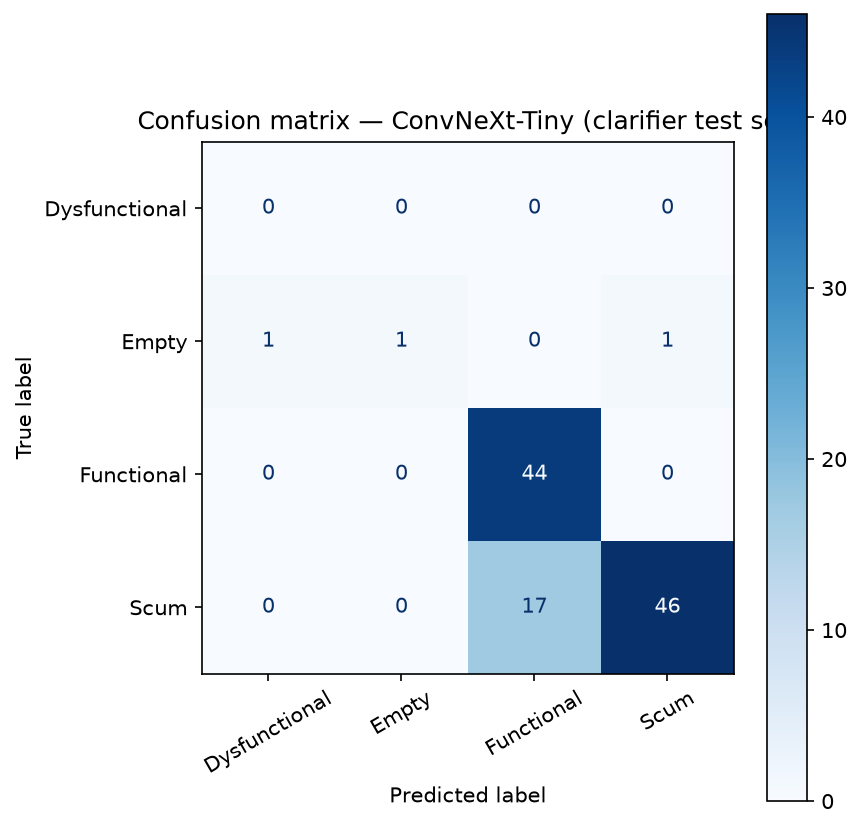
\includegraphics[width=\textwidth]{figures/results/clarifier_convnext_tiny_Atlantis_confusion_matrix.png}
        \caption{Atlantis}
    \end{subfigure}
    \hfill
    \begin{subfigure}{0.32\textwidth}
        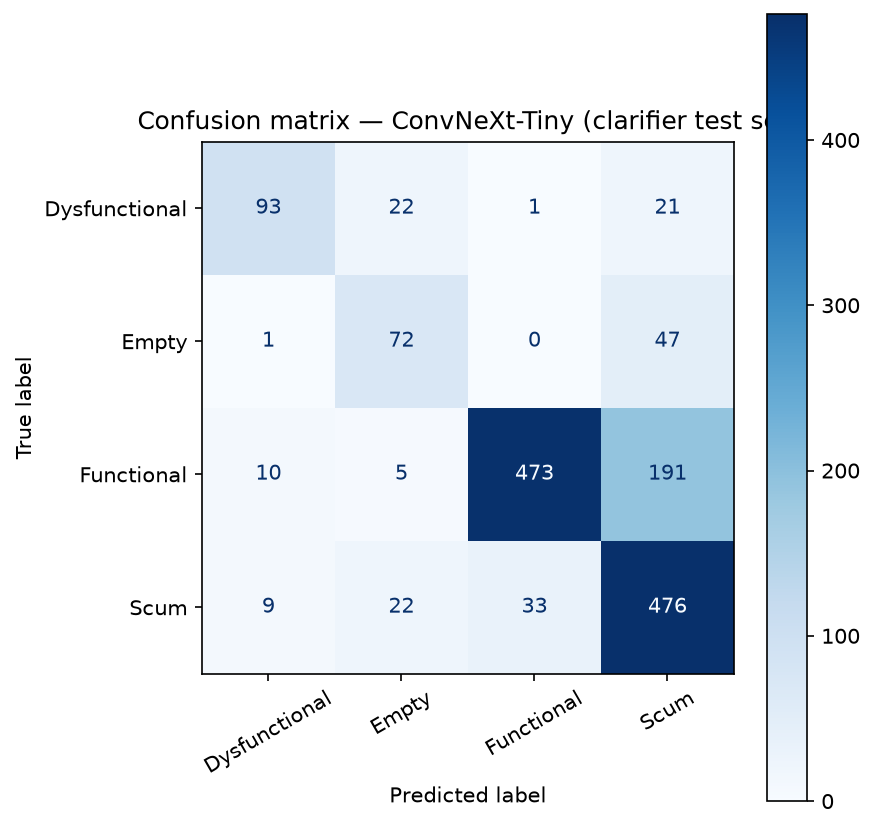
\includegraphics[width=\textwidth]{figures/results/clarifier_convnext_tiny_CapeFlats_confusion_matrix.png}
        \caption{Cape Flats}
    \end{subfigure}
    \hfill
    \begin{subfigure}{0.32\textwidth}
        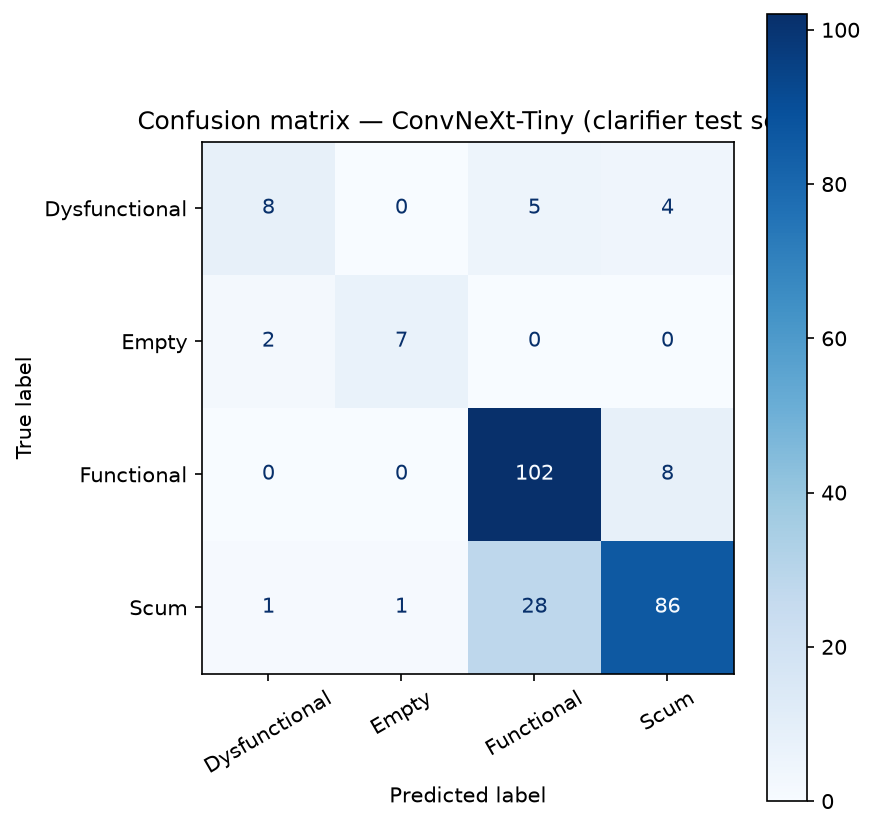
\includegraphics[width=\textwidth]{figures/results/clarifier_convnext_tiny_Fisantekraal_confusion_matrix.png}
        \caption{Fisantekraal}
    \end{subfigure}
    \begin{subfigure}{0.32\textwidth}
        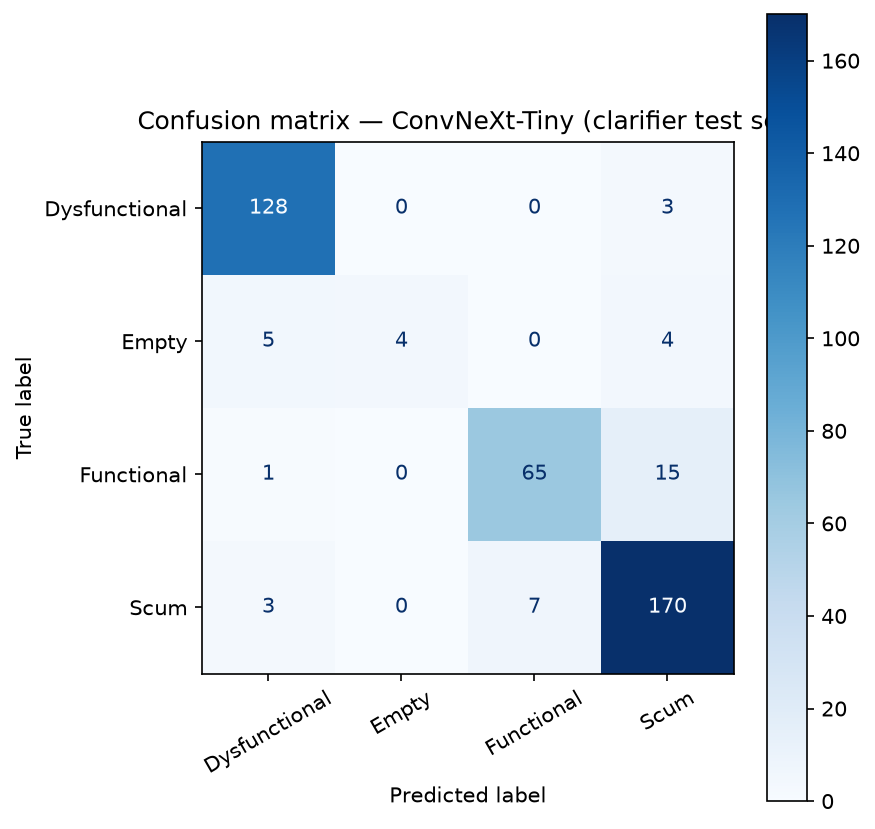
\includegraphics[width=\textwidth]{figures/results/clarifier_convnext_tiny_NoordelikeWerke_confusion_matrix.png}
        \caption{Northern Works}
    \end{subfigure}
    \begin{subfigure}{0.32\textwidth}
        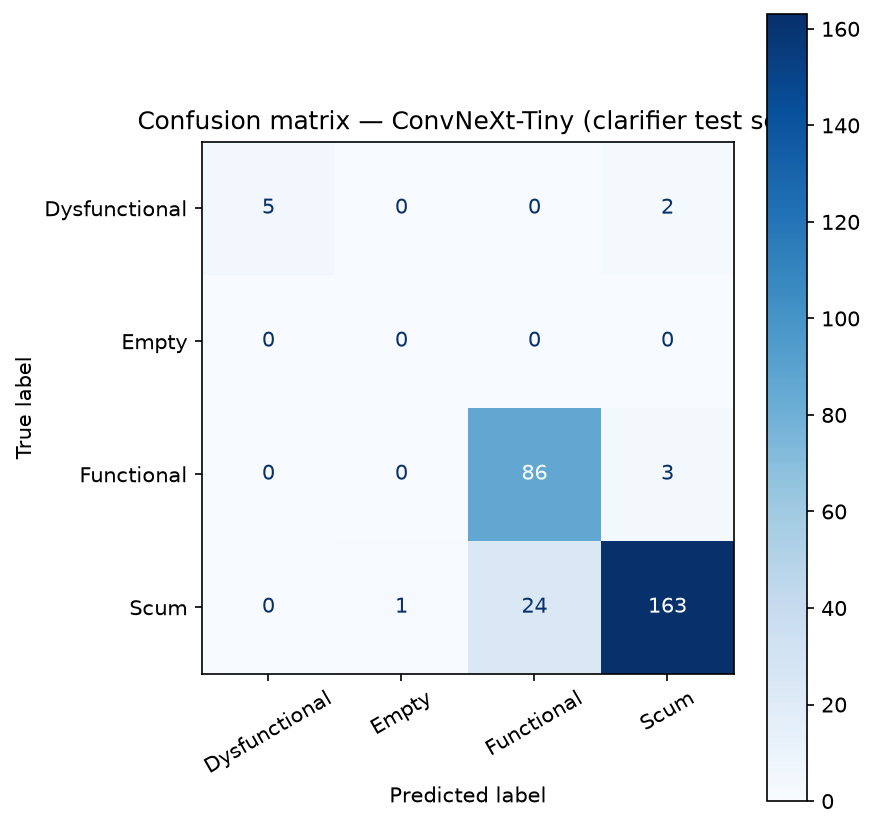
\includegraphics[width=\textwidth]{figures/results/clarifier_convnext_tiny_Waterval_confusion_matrix.png}
        \caption{Waterval}
    \end{subfigure}
    \caption{Confusion matrices of the ConvNeXt-Tiny clarifier model on each held-out facility.}
    \label{fig:res_lofo_clarifier_cm}
\end{figure}

Figure~\ref{fig:res_lofo_clarifier_cm} shows that the most common mistake at every facility is a confusion between \textbf{Scum} and \textbf{Functional}. At Atlantis, Fisantekraal and Waterval, 17 of 63, 28 of 116 and 24 of 188 \textbf{Scum} clarifiers are classified as \textbf{Functional}. At Cape Flats and Northern Works the direction is reversed: 191 of 679 and 15 of 81 \textbf{Functional} clarifiers are classified as \textbf{Scum}. At Cape Flats, 47 of the 120 \textbf{Empty} clarifiers are also classified as \textbf{Scum}.

\begin{table}[htbp]
\centering
\small
\setlength{\tabcolsep}{4pt}
\caption{Aerobic zone test results of every architecture in the leave-one-facility-out experiment (Experiment~2), given as the mean $\pm$ standard deviation across the three held-out facilities.}
\label{tab:res_lofo_aerobic}
\resizebox{\textwidth}{!}{%
\begin{tabular}{lrrrrr}
\toprule
\textbf{Architecture} & \textbf{Accuracy} & \textbf{Mean AUC} & \textbf{\makecell[r]{Macro\\precision}} & \textbf{\makecell[r]{Macro\\recall}} & \textbf{\makecell[r]{Macro\\F1}} \\
\midrule
ResNet-18 & 0.598 $\pm$ 0.052 & 0.694 $\pm$ 0.057 & 0.438 $\pm$ 0.070 & 0.517 $\pm$ 0.029 & 0.435 $\pm$ 0.081 \\
EfficientNet-B0 & 0.529 $\pm$ 0.255 & 0.705 $\pm$ 0.054 & 0.487 $\pm$ 0.051 & 0.484 $\pm$ 0.040 & 0.413 $\pm$ 0.130 \\
DenseNet-121 & \textbf{0.628} $\pm$ 0.096 & \textbf{0.763} $\pm$ 0.025 & 0.498 $\pm$ 0.025 & \textbf{0.541} $\pm$ 0.028 & \textbf{0.495} $\pm$ 0.033 \\
ResNet-50 & 0.561 $\pm$ 0.163 & 0.692 $\pm$ 0.007 & 0.439 $\pm$ 0.029 & 0.476 $\pm$ 0.034 & 0.402 $\pm$ 0.073 \\
ConvNeXt-Tiny & 0.540 $\pm$ 0.219 & 0.758 $\pm$ 0.088 & \textbf{0.514} $\pm$ 0.114 & 0.537 $\pm$ 0.116 & 0.451 $\pm$ 0.194 \\
Inception-v3 & 0.577 $\pm$ 0.046 & 0.711 $\pm$ 0.095 & 0.473 $\pm$ 0.037 & 0.491 $\pm$ 0.063 & 0.426 $\pm$ 0.034 \\
ResNet-18 (scratch) & 0.389 $\pm$ 0.155 & 0.624 $\pm$ 0.023 & 0.441 $\pm$ 0.029 & 0.399 $\pm$ 0.028 & 0.331 $\pm$ 0.101 \\
\bottomrule
\end{tabular}}
\end{table}

Table~\ref{tab:res_lofo_aerobic} shows that DenseNet-121 has the highest mean accuracy, mean AUC, macro recall and macro F1 score, and ConvNeXt-Tiny the highest macro precision. The standard deviation of the macro F1 score ranges from 0.033 (DenseNet-121) to 0.194 (ConvNeXt-Tiny), and that of the accuracy from 0.046 (Inception-v3) to 0.255 (EfficientNet-B0). The accuracy of ResNet-18 (scratch) is 0.389, which is 0.140 below the lowest accuracy of a pretrained model.

\begin{table}[htbp]
\centering
\small
\caption{Aerobic zone test accuracy and mean AUC of every architecture for each held-out facility.}
\label{tab:res_lofo_aerobic_facility}
\begin{tabular}{lrrrr}
\toprule
\textbf{Architecture} & \textbf{Atlantis} & \textbf{Cape Flats} & \textbf{Waterval} & \textbf{Mean} \\
\midrule
\multicolumn{5}{l}{\textit{Accuracy}} \\
ResNet-18 & 0.619 & 0.538 & 0.635 & 0.598 \\
EfficientNet-B0 & 0.611 & 0.243 & 0.734 & 0.529 \\
DenseNet-121 & 0.575 & \textbf{0.570} & \textbf{0.740} & \textbf{0.628} \\
ResNet-50 & \textbf{0.637} & 0.375 & 0.672 & 0.561 \\
ConvNeXt-Tiny & 0.593 & 0.300 & 0.728 & 0.540 \\
Inception-v3 & 0.558 & 0.543 & 0.630 & 0.577 \\
ResNet-18 (scratch) & 0.469 & 0.210 & 0.487 & 0.389 \\
\midrule
\multicolumn{5}{l}{\textit{Mean AUC}} \\
ResNet-18 & 0.697 & 0.636 & 0.750 & 0.694 \\
EfficientNet-B0 & 0.715 & 0.647 & 0.753 & 0.705 \\
DenseNet-121 & 0.736 & 0.770 & 0.783 & \textbf{0.763} \\
ResNet-50 & 0.700 & 0.687 & 0.690 & 0.692 \\
ConvNeXt-Tiny & \textbf{0.820} & 0.656 & \textbf{0.796} & 0.758 \\
Inception-v3 & 0.602 & \textbf{0.771} & 0.761 & 0.711 \\
ResNet-18 (scratch) & 0.645 & 0.628 & 0.600 & 0.624 \\
\bottomrule
\end{tabular}
\end{table}

Table~\ref{tab:res_lofo_aerobic_facility} shows that Cape Flats has the lowest accuracy of every architecture, from 0.210 to 0.570. Most aerobic zones at Cape Flats are \textbf{Dysfunctional} (562 of 766, Figure~\ref{fig:res_lofo_aerobic_cm}), so the accuracy there depends mainly on the \textbf{Dysfunctional} recall. EfficientNet-B0 and ConvNeXt-Tiny, the pretrained models with the lowest accuracy at Cape Flats (0.243 and 0.300), also have the largest standard deviation of the accuracy in Table~\ref{tab:res_lofo_aerobic}. The mean AUC does not follow the same pattern: for DenseNet-121 and Inception-v3, the AUC at Cape Flats is higher than at Atlantis.

\begin{table}[htbp]
\centering
\small
\setlength{\tabcolsep}{4pt}
\caption{Per-class precision (P), recall (R) and F1 score of every aerobic zone architecture in Experiment~2, averaged over the three held-out facilities.}
\label{tab:res_lofo_aerobic_perclass}
\resizebox{\textwidth}{!}{%
\begin{tabular}{l rrr rrr rrr}
\toprule
& \multicolumn{3}{c}{\textbf{Dysfunctional}} & \multicolumn{3}{c}{\textbf{Functional}} & \multicolumn{3}{c}{\textbf{Suboptimal}} \\
\cmidrule(lr){2-4} \cmidrule(lr){5-7} \cmidrule(lr){8-10}
\textbf{Architecture} & P & R & F1 & P & R & F1 & P & R & F1 \\
\midrule
ResNet-18 & 0.609 & \textbf{0.726} & 0.616 & 0.647 & 0.752 & 0.625 & 0.057 & 0.072 & 0.064 \\
EfficientNet-B0 & 0.703 & 0.458 & 0.451 & 0.628 & 0.796 & 0.669 & 0.130 & 0.198 & 0.118 \\
DenseNet-121 & 0.696 & 0.712 & \textbf{0.680} & \textbf{0.675} & 0.728 & 0.664 & 0.124 & 0.184 & 0.141 \\
ResNet-50 & 0.662 & 0.509 & 0.510 & 0.588 & \textbf{0.865} & 0.646 & 0.066 & 0.055 & 0.050 \\
ConvNeXt-Tiny & \textbf{0.712} & 0.593 & 0.550 & 0.639 & 0.793 & 0.599 & \textbf{0.192} & 0.224 & \textbf{0.203} \\
Inception-v3 & 0.640 & 0.525 & 0.469 & 0.672 & 0.746 & \textbf{0.671} & 0.105 & 0.202 & 0.137 \\
ResNet-18 (scratch) & 0.637 & 0.244 & 0.280 & 0.558 & 0.659 & 0.537 & 0.128 & \textbf{0.294} & 0.177 \\
\bottomrule
\end{tabular}}
\end{table}

Table~\ref{tab:res_lofo_aerobic_perclass} shows that the \textbf{Suboptimal} recall ranges from 0.055 to 0.294 and the \textbf{Suboptimal} F1 score from 0.050 to 0.203. The \textbf{Dysfunctional} recall ranges from 0.244 to 0.726, against 0.811 to 0.940 in Experiment~1 (Table~\ref{tab:res_mixed_aerobic_perclass}).

\begin{figure}[htbp]
    \centering
    \begin{subfigure}{0.49\textwidth}
        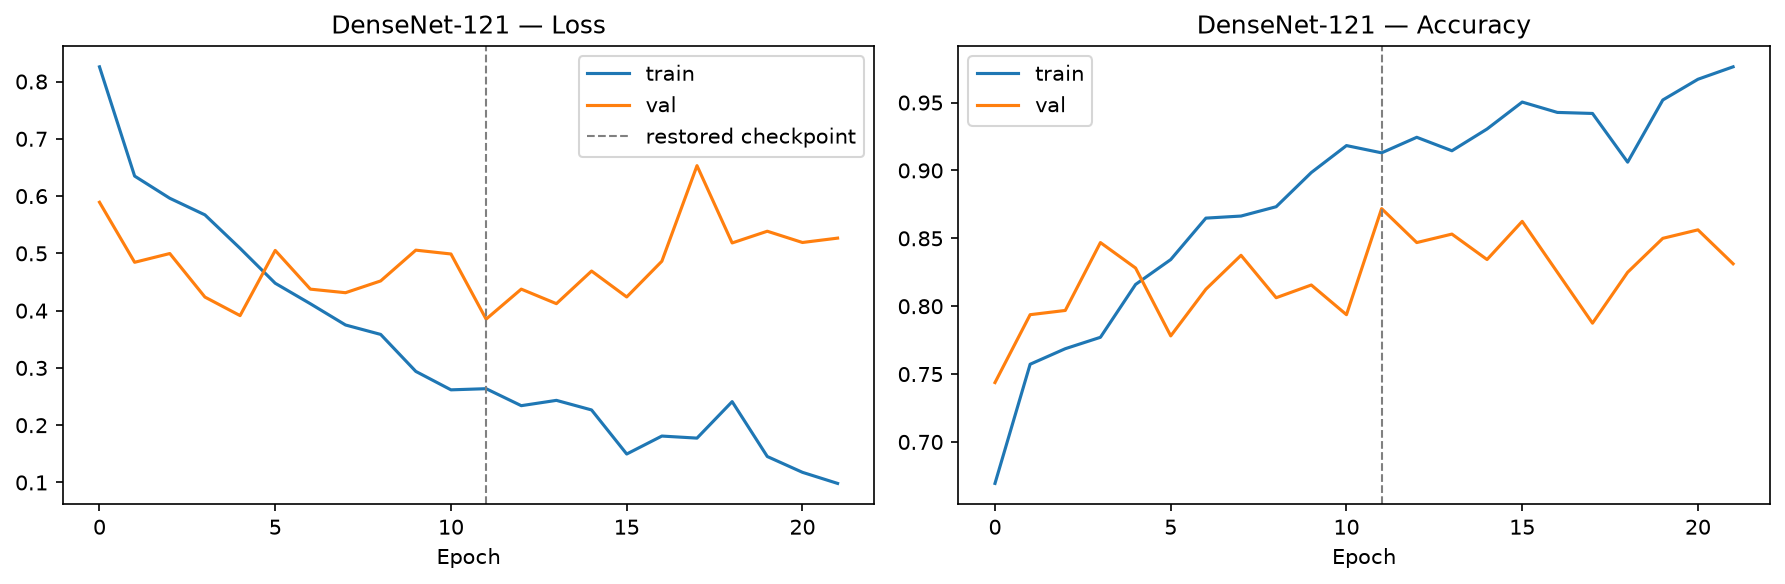
\includegraphics[width=\textwidth]{figures/results/aerobic_zone_densenet_121_Atlantis_training_curves.png}
        \caption{Atlantis held out}
    \end{subfigure}
    \hfill
    \begin{subfigure}{0.49\textwidth}
        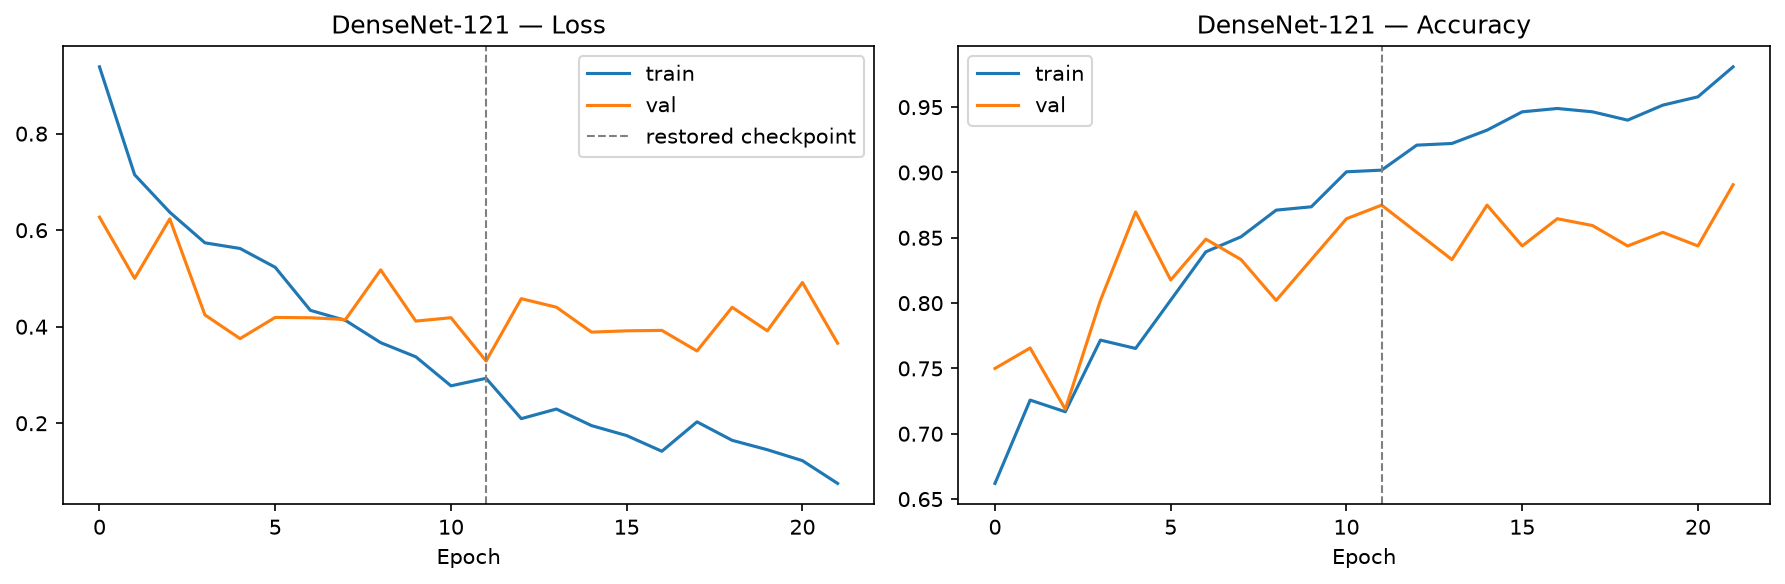
\includegraphics[width=\textwidth]{figures/results/aerobic_zone_densenet_121_CapeFlats_training_curves.png}
        \caption{Cape Flats held out}
    \end{subfigure}
    \begin{subfigure}{0.49\textwidth}
        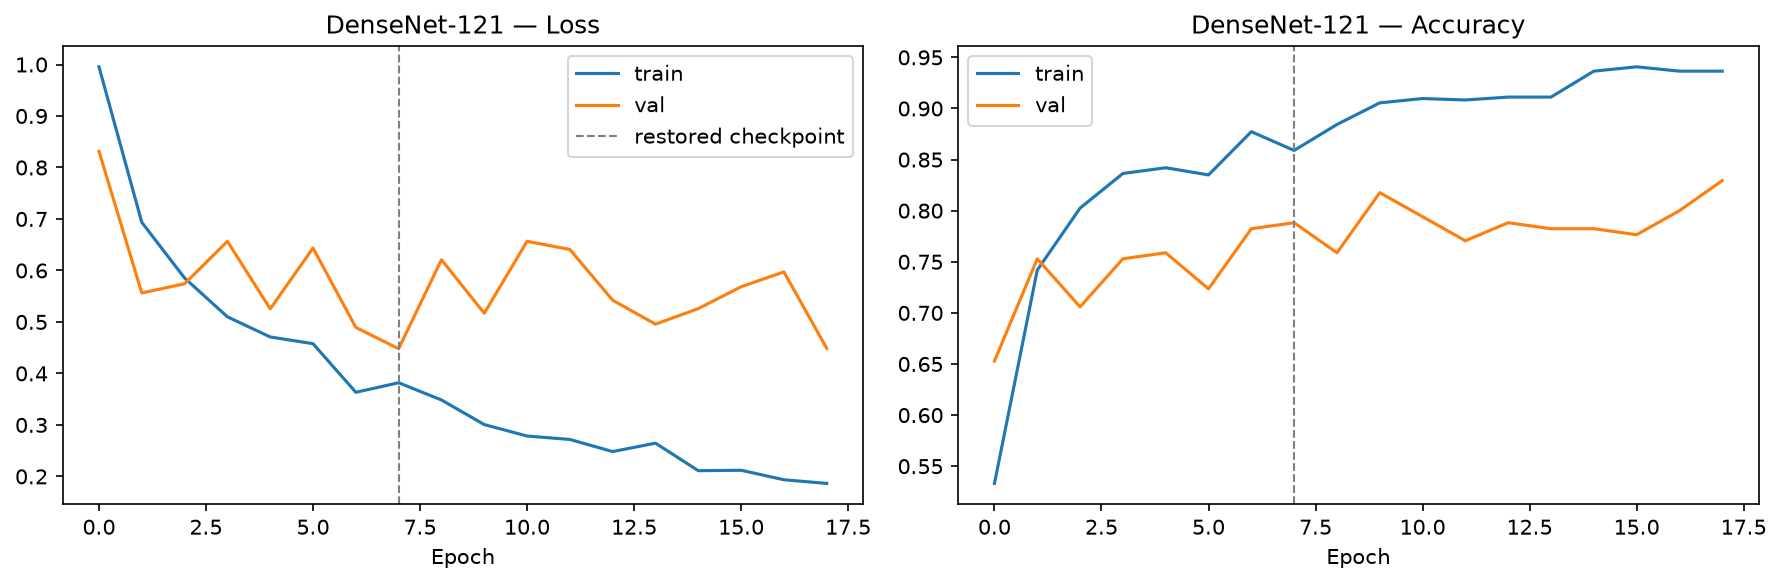
\includegraphics[width=\textwidth]{figures/results/aerobic_zone_densenet_121_Waterval_training_curves.png}
        \caption{Waterval held out}
    \end{subfigure}
    \caption{Training and development loss and accuracy of the DenseNet-121 aerobic zone model for every leave-one-facility-out fold. The dashed line marks the epoch of the restored checkpoint.}
    \label{fig:res_lofo_aerobic_curves}
\end{figure}

Figure~\ref{fig:res_lofo_aerobic_curves} shows that the development loss of every fold stops decreasing after 8 to 12 epochs, and training stops 10 epochs later. The development loss varies more from epoch to epoch than for the clarifiers. At the checkpoint, the development accuracy is about 0.79 to 0.87, while the test accuracy at the held-out facility is 0.570 to 0.740 (Table~\ref{tab:res_lofo_aerobic_facility}). The development accuracy therefore overestimates the accuracy at a new facility.

\begin{figure}[htbp]
    \centering
    \begin{subfigure}{0.32\textwidth}
        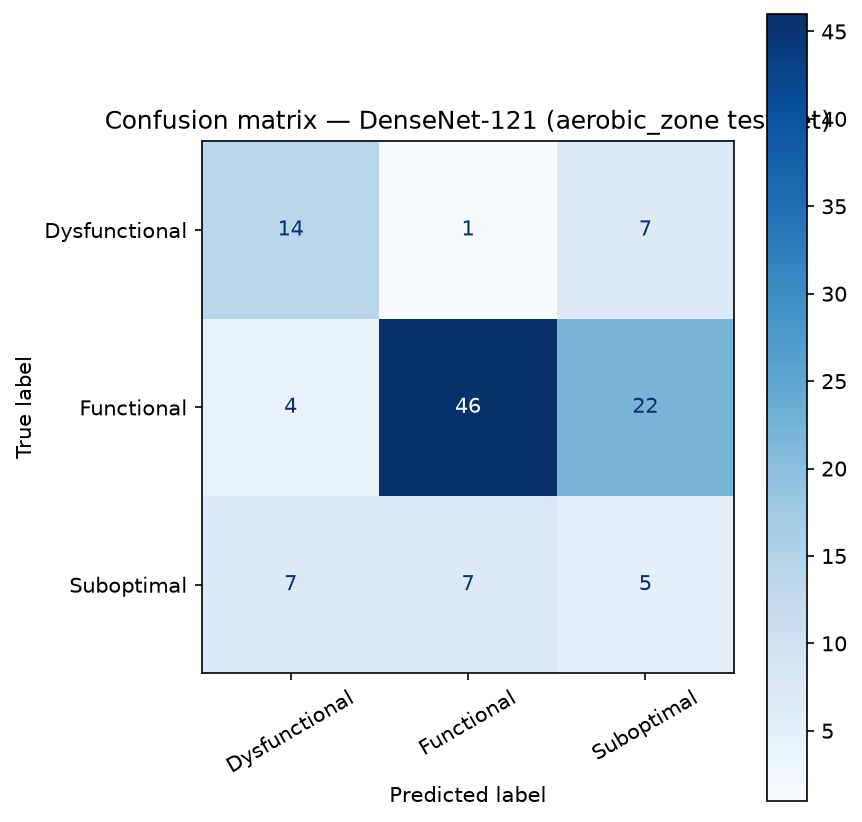
\includegraphics[width=\textwidth]{figures/results/aerobic_zone_densenet_121_Atlantis_confusion_matrix.png}
        \caption{Atlantis}
    \end{subfigure}
    \hfill
    \begin{subfigure}{0.32\textwidth}
        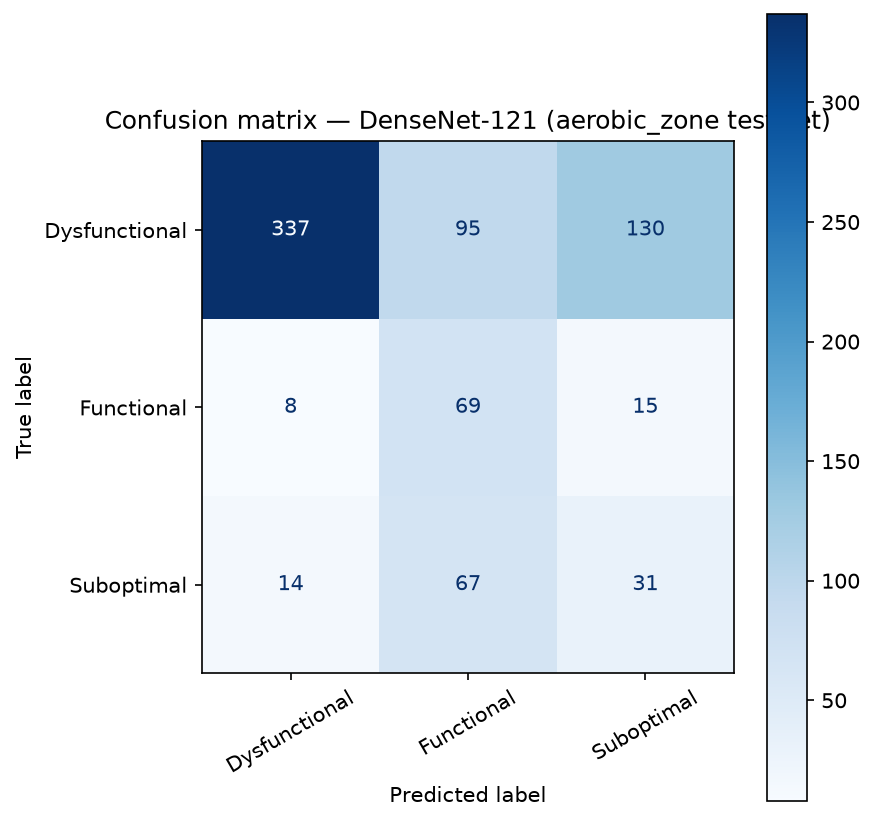
\includegraphics[width=\textwidth]{figures/results/aerobic_zone_densenet_121_CapeFlats_confusion_matrix.png}
        \caption{Cape Flats}
    \end{subfigure}
    \hfill
    \begin{subfigure}{0.32\textwidth}
        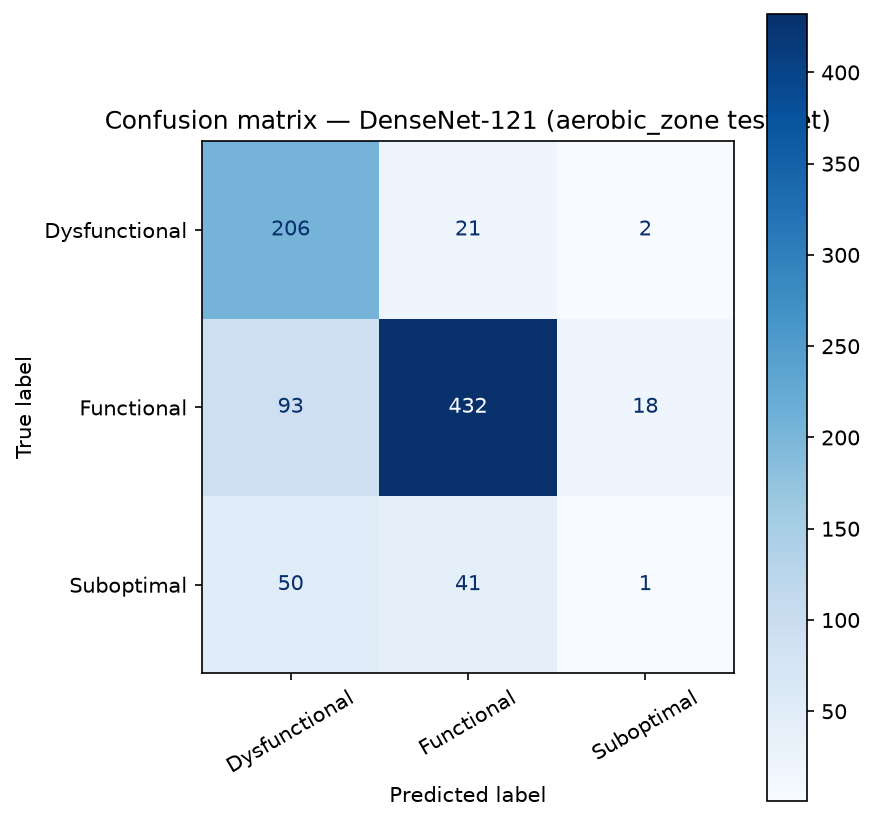
\includegraphics[width=\textwidth]{figures/results/aerobic_zone_densenet_121_Waterval_confusion_matrix.png}
        \caption{Waterval}
    \end{subfigure}
    \caption{Confusion matrices of the DenseNet-121 aerobic zone model on each held-out facility.}
    \label{fig:res_lofo_aerobic_cm}
\end{figure}

Figure~\ref{fig:res_lofo_aerobic_cm} shows that the most common mistake differs between facilities. At Atlantis, 22 of the 72 \textbf{Functional} zones are classified as \textbf{Suboptimal}. At Cape Flats, 130 and 95 of the 562 \textbf{Dysfunctional} zones are classified as \textbf{Suboptimal} and \textbf{Functional}, and 67 of the 112 \textbf{Suboptimal} zones as \textbf{Functional}. At Waterval, 93 of the 543 \textbf{Functional} zones are classified as \textbf{Dysfunctional}, and only 1 of the 92 \textbf{Suboptimal} zones is classified correctly.

\FloatBarrier

\section{Effect of Augmentation}
\label{sec:results_augmentation}

Table~\ref{tab:res_augmentation} compares the chronological-split results of every architecture trained with and without the augmentations described in Section~\ref{sec:exp_augmentation}.

\begin{table}[htbp]
\centering
\small
\setlength{\tabcolsep}{4pt}
\caption{Test results on the chronological split with (Aug.) and without (None) augmentation during training. $\Delta$ is the difference in percentage points, where a positive value means that augmentation helped.}
\label{tab:res_augmentation}
\begin{tabular}{l rrr rrr rr}
\toprule
& \multicolumn{3}{c}{\textbf{Accuracy}} & \multicolumn{3}{c}{\textbf{Macro F1}} & \multicolumn{2}{c}{\textbf{Mean AUC}} \\
\cmidrule(lr){2-4} \cmidrule(lr){5-7} \cmidrule(lr){8-9}
\textbf{Architecture} & Aug. & None & $\Delta$ & Aug. & None & $\Delta$ & Aug. & None \\
\midrule
\multicolumn{9}{l}{\textit{Clarifiers}} \\
ResNet-18 & 0.776 & 0.745 & +3.1 & 0.732 & 0.684 & +4.8 & 0.929 & 0.913 \\
EfficientNet-B0 & 0.780 & 0.789 & -0.9 & 0.691 & 0.721 & -3.0 & 0.927 & 0.921 \\
DenseNet-121 & 0.785 & 0.777 & +0.8 & 0.772 & 0.703 & +6.9 & 0.926 & 0.919 \\
ResNet-50 & 0.761 & 0.687 & +7.4 & 0.702 & 0.593 & +10.9 & 0.922 & 0.888 \\
ConvNeXt-Tiny & 0.838 & 0.798 & +4.0 & 0.748 & 0.736 & +1.2 & 0.949 & 0.950 \\
Inception-v3 & 0.773 & 0.770 & +0.3 & 0.706 & 0.712 & -0.6 & 0.926 & 0.903 \\
ResNet-18 (scratch) & 0.713 & 0.655 & +5.8 & 0.667 & 0.605 & +6.2 & 0.904 & 0.857 \\
\midrule
\multicolumn{9}{l}{\textit{Aerobic zones}} \\
ResNet-18 & 0.806 & 0.810 & -0.4 & 0.638 & 0.599 & +3.9 & 0.860 & 0.885 \\
EfficientNet-B0 & 0.857 & 0.808 & +4.9 & 0.740 & 0.641 & +9.9 & 0.924 & 0.849 \\
DenseNet-121 & 0.813 & 0.852 & -3.9 & 0.662 & 0.693 & -3.1 & 0.898 & 0.925 \\
ResNet-50 & 0.815 & 0.737 & +7.8 & 0.653 & 0.608 & +4.5 & 0.900 & 0.845 \\
ConvNeXt-Tiny & 0.850 & 0.843 & +0.7 & 0.724 & 0.744 & -2.0 & 0.938 & 0.940 \\
Inception-v3 & 0.820 & 0.795 & +2.5 & 0.687 & 0.678 & +0.9 & 0.903 & 0.917 \\
ResNet-18 (scratch) & 0.781 & 0.776 & +0.5 & 0.624 & 0.584 & +4.0 & 0.893 & 0.811 \\
\bottomrule
\end{tabular}
\end{table}

Table~\ref{tab:res_augmentation} shows that augmentation increased the clarifier accuracy of six of the seven models, all except EfficientNet-B0, and the clarifier macro F1 score of five. For the aerobic zones, it increased the macro F1 score of five models, but decreased the accuracy and macro F1 score of DenseNet-121 by 3.9 and 3.1 percentage points. The largest increases in macro F1 score are 10.9 percentage points for the ResNet-50 clarifiers and 9.9 for the EfficientNet-B0 aerobic zones.

\FloatBarrier

\section{Binary (OK / Not-OK) Results}
\label{appen:res_binary}

Table~\ref{tab:res_threshold} gives the threshold chosen on the development set for every architecture, with the test recall of the Not-OK class at that threshold. Tables~\ref{tab:res_threshold_robustness_clarifier} and~\ref{tab:res_threshold_robustness_aerobic} give the recall and specificity for every held-out facility at the threshold of that fold.

\begin{table}[htbp]
\centering
\small
\setlength{\tabcolsep}{4pt}
\caption{Threshold $t$ on the Not-OK score chosen for a 95\% recall on the development set, with the test recall of the Not-OK class at that threshold. For the leave-one-facility-out split, every fold has its own threshold, and the threshold and recall are averaged across held-out facilities. The specificity and precision at these thresholds are given in Table~\ref{tab:res_binary} (Section~\ref{sec:results_binary}).}
\label{tab:res_threshold}
\begin{tabular}{l rr rr}
\toprule
& \multicolumn{2}{c}{\textbf{Chronological}} & \multicolumn{2}{c}{\textbf{Leave-one-facility-out}} \\
\cmidrule(lr){2-3} \cmidrule(lr){4-5}
\textbf{Architecture} & $t$ & Recall & $t$ & Recall \\
\midrule
\multicolumn{5}{l}{\textit{Clarifiers}} \\
ResNet-18 & 0.244 & 0.974 & 0.280 & 0.867 \\
EfficientNet-B0 & 0.194 & 0.961 & 0.328 & 0.902 \\
DenseNet-121 & 0.309 & 0.959 & 0.309 & 0.897 \\
ResNet-50 & 0.160 & 0.983 & 0.267 & 0.915 \\
ConvNeXt-Tiny & 0.126 & 0.968 & 0.353 & 0.886 \\
Inception-v3 & 0.134 & 0.966 & 0.236 & 0.900 \\
ResNet-18 (scratch) & 0.140 & 0.964 & 0.238 & 0.916 \\
\midrule
\multicolumn{5}{l}{\textit{Aerobic zones}} \\
ResNet-18 & 0.541 & 0.931 & 0.312 & 0.846 \\
EfficientNet-B0 & 0.257 & 0.941 & 0.400 & 0.740 \\
DenseNet-121 & 0.585 & 0.924 & 0.387 & 0.864 \\
ResNet-50 & 0.309 & 0.894 & 0.321 & 0.703 \\
ConvNeXt-Tiny & 0.313 & 0.950 & 0.552 & 0.692 \\
Inception-v3 & 0.437 & 0.950 & 0.434 & 0.878 \\
ResNet-18 (scratch) & 0.455 & 0.881 & 0.475 & 0.719 \\
\bottomrule
\end{tabular}
\end{table}

Table~\ref{tab:res_threshold} shows that the chosen threshold differs between architectures, from 0.126 to 0.585 on the chronological split and from 0.236 to 0.552 as a mean across folds in the leave-one-facility-out experiment. The thresholds of the individual folds range from 0.114 to 0.591 for the clarifiers and from 0.208 to 0.834 for the aerobic zones.

\begin{table}[htbp]
\centering
\small
\setlength{\tabcolsep}{4pt}
\caption{Recall and specificity of the Not-OK class for each held-out facility at the clarifier threshold chosen on the development set of that fold, with the lowest recall and the standard deviation of the recall across facilities.}
\label{tab:res_threshold_robustness_clarifier}
\resizebox{\textwidth}{!}{%
\begin{tabular}{l rrrrr rr}
\toprule
\textbf{Architecture} & \textbf{Atlantis} & \textbf{\makecell[r]{Cape\\Flats}} & \textbf{\makecell[r]{Fisante-\\kraal}} & \textbf{\makecell[r]{Northern\\Works}} & \textbf{Waterval} & \textbf{Min.} & \textbf{Std.} \\
\midrule
\multicolumn{8}{l}{\textit{Recall}} \\
ResNet-18 & 0.667 & 0.987 & 0.732 & 0.988 & 0.959 & 0.667 & 0.155 \\
EfficientNet-B0 & 0.818 & 0.969 & 0.768 & 0.981 & 0.974 & 0.768 & 0.101 \\
DenseNet-121 & 0.788 & 0.990 & 0.803 & 0.963 & 0.944 & 0.788 & 0.095 \\
ResNet-50 & 0.818 & 0.985 & 0.824 & 0.997 & 0.949 & 0.818 & 0.087 \\
ConvNeXt-Tiny & 0.758 & 0.956 & 0.810 & 0.985 & 0.923 & 0.758 & 0.098 \\
Inception-v3 & 0.727 & 0.979 & 0.880 & 0.991 & 0.923 & 0.727 & 0.106 \\
ResNet-18 (scratch) & 0.848 & 0.962 & 0.831 & 1.000 & 0.938 & 0.831 & 0.073 \\
\midrule
\multicolumn{8}{l}{\textit{Specificity}} \\
ResNet-18 & 0.955 & 0.187 & 0.818 & 0.247 & 0.494 \\
EfficientNet-B0 & 0.977 & 0.297 & 0.891 & 0.679 & 0.663 \\
DenseNet-121 & 0.977 & 0.236 & 0.845 & 0.741 & 0.753 \\
ResNet-50 & 0.955 & 0.166 & 0.864 & 0.506 & 0.674 \\
ConvNeXt-Tiny & 1.000 & 0.704 & 0.882 & 0.790 & 0.854 \\
Inception-v3 & 0.977 & 0.206 & 0.582 & 0.272 & 0.764 \\
ResNet-18 (scratch) & 0.909 & 0.174 & 0.700 & 0.049 & 0.708 \\
\bottomrule
\end{tabular}}
\end{table}

Table~\ref{tab:res_threshold_robustness_clarifier} shows that the lowest clarifier recall of every architecture occurs at Atlantis or Fisantekraal, and ranges from 0.667 to 0.831. At these two facilities the specificity is 0.582 to 1.000, so the threshold flags too few components there. At Cape Flats and Northern Works the recall is at least 0.956, and at Cape Flats the specificity is at most 0.297 for every architecture except ConvNeXt-Tiny (0.704), so most OK clarifiers there are flagged.

\begin{table}[htbp]
\centering
\small
\caption{Recall and specificity of the Not-OK class for each held-out facility at the aerobic zone threshold chosen on the development set of that fold, with the lowest recall and the standard deviation of the recall across facilities.}
\label{tab:res_threshold_robustness_aerobic}
\begin{tabular}{l rrr rr}
\toprule
\textbf{Architecture} & \textbf{Atlantis} & \textbf{Cape Flats} & \textbf{Waterval} & \textbf{Min.} & \textbf{Std.} \\
\midrule
\multicolumn{6}{l}{\textit{Recall}} \\
ResNet-18 & 0.976 & 0.760 & 0.804 & 0.760 & 0.114 \\
EfficientNet-B0 & 0.902 & 0.795 & 0.523 & 0.523 & 0.195 \\
DenseNet-121 & 0.878 & 0.935 & 0.779 & 0.779 & 0.079 \\
ResNet-50 & 0.902 & 0.780 & 0.427 & 0.427 & 0.247 \\
ConvNeXt-Tiny & 0.951 & 0.447 & 0.679 & 0.447 & 0.253 \\
Inception-v3 & 0.927 & 0.958 & 0.748 & 0.748 & 0.114 \\
ResNet-18 (scratch) & 0.829 & 0.782 & 0.545 & 0.545 & 0.152 \\
\midrule
\multicolumn{6}{l}{\textit{Specificity}} \\
ResNet-18 & 0.458 & 0.663 & 0.599 \\
EfficientNet-B0 & 0.500 & 0.685 & 0.917 \\
DenseNet-121 & 0.444 & 0.554 & 0.808 \\
ResNet-50 & 0.528 & 0.783 & 0.849 \\
ConvNeXt-Tiny & 0.667 & 0.978 & 0.849 \\
Inception-v3 & 0.597 & 0.391 & 0.750 \\
ResNet-18 (scratch) & 0.472 & 0.685 & 0.516 \\
\bottomrule
\end{tabular}
\end{table}

Table~\ref{tab:res_threshold_robustness_aerobic} shows that the lowest aerobic zone recall ranges from 0.427 to 0.779, and occurs at Waterval for five of the seven architectures. The target of 95\% is reached in only 3 of the 21 combinations of architecture and facility. DenseNet-121 has the smallest standard deviation of the recall (0.079, against 0.114 to 0.253) and the highest lowest recall. ConvNeXt-Tiny, which has the highest binary AUC in Experiment~2 (Table~\ref{tab:res_binary} in Section~\ref{sec:results_binary}), has a recall of 0.447 at Cape Flats.

\FloatBarrier